\documentclass[12pt,twoside]{book}

\usepackage[a4paper,inner=3.5cm,outer=2.5cm,top=2.5cm,bottom=2.5cm]{geometry}
\usepackage{fontspec}
\usepackage{polski}
\usepackage[polish]{babel}
\usepackage{setspace}
\usepackage{fancyhdr}
\usepackage{titlesec}

\setmainfont{Times New Roman}
\setstretch{1.5}
\pagestyle{fancy}
\fancyhf{}
\fancyfoot[CE,CO]{\thepage}
\renewcommand{\headrulewidth}{0pt}
\fancypagestyle{plain}{%
  \fancyhf{}%
  \renewcommand{\headrulewidth}{0pt}%
  \fancyfoot[CE,CO]{\thepage}%
}



% Konfiguracja nagłówków
% Nagłówek 1. stopnia: 12 pkt, WERSALIKI, pogrubiona
\titleformat{\chapter}[hang]
  {\normalfont\bfseries\fontsize{12}{14}\selectfont\uppercase}
  {\thechapter.}
  {1em}
  {}
  
% Nagłówek 2. stopnia: 10 pkt, pogrubiona i kursywa
\titleformat{\section}
  {\normalfont\bfseries\itshape\fontsize{10}{12}\selectfont}
  {\thesection}
  {1em}
  {}

% Nagłówek 3. stopnia: 10 pkt, kursywa
\titleformat{\subsection}
  {\normalfont\itshape\fontsize{10}{12}\selectfont}
  {\thesubsection}
  {1em}
  {}

% Dostosowanie odstępów dla nagłówków
\titlespacing*{\chapter}{0pt}{12pt}{6pt}
\titlespacing*{\section}{0pt}{12pt}{6pt}
\titlespacing*{\subsection}{0pt}{12pt}{6pt}

\usepackage{lipsum}
\usepackage{pdfpages}
\usepackage{tocloft}
\usepackage{cite}
\usepackage{indentfirst}
\usepackage{enumitem}
\usepackage{graphicx}
\usepackage[font=normalsize,labelfont=bf]{caption} % Konfiguracja podpisów
\usepackage[hidelinks]{hyperref}

\renewcommand{\contentsname}{Spis treści}
\renewcommand{\cftchapleader}{\cftdotfill{\cftdotsep}}
\renewcommand{\cfttoctitlefont}{\bfseries\fontsize{12pt}{14pt}\selectfont}
\renewcommand{\cftloftitlefont}{\bfseries\fontsize{12pt}{14pt}\selectfont}

\setlength{\parindent}{1.25cm}

\captionsetup[figure]{
  labelsep=period, % Ustawienie kropki zamiast dwukropka
  justification=centering, % Wyśrodkowanie podpisu
  font=normalsize, % Rozmiar czcionki podpisu
  textfont=normalfont, % Styl czcionki podpisu
  labelfont=normalfont, % Pogrubienie etykiety "Rys."
  name=Rys., % Zmiana nazwy "Rysunek" na "Rys."
  skip=12pt %Ustawienie dolnego odstępu podpisu
}

% Dodanie odstępu przed podpisem rysunku
\newcommand{\captionvspace}{\vspace{6pt}}

% Dostosowanie odstępów dla środowiska 'itemize'
\setlist[itemize]{topsep=0pt,partopsep=0pt}

\begin{document}

\setcounter{page}{1}
\thispagestyle{empty}
\includepdf{includes/pdf/strona_tytułowa.pdf}

% Tutaj umieść swoją stronę ze spisem treści
\tableofcontents

% Tutaj zaczyna się główna treść pracy
\chapter{Wstęp}

\section{Cel pracy}

Celem niniejszej pracy dyplomowej jest zbadanie procesu migracji systemu monolitycznego do architektury mikroserwisowej opartej o usługi chmury obliczeniowej dostawcy Amazon Web Services (w skrócie AWS) pod kątem ulepszenia zabezpieczeń omawianego systemu. System objęty badaniem, to: „System do internetowego wspomagania pacjenta i lekarza”, który został w całości zaprojektowany i zaimplementowany w formie monolitycznej przez autora pracy dyplomowej jako projekt inżynierski w celu ukończenia studiów inżynierskich pierwszego stopnia. Wybór systemu do przeprowadzenia analizy motywowany jest znajomością jego architektury, wpasowującą się doskonale w temat pracy oraz motywacja do jego dalszego rozwijania i ulepszania w zakresie cyberbezpieczeństwa.

Analiza procesu migracji oraz rozwinięcia systemu zabezpieczeń systemu ma wykazać jak dobrze usługi chmurowe ochraniają swoich usługobiorców i ich oprogramowania przed popularnymi atakami hakerskimi oraz jak duży wpływ na bezpieczeństwo systemu ma jego architektura. Narzędzia używane przez autor pracy to przede wszystkim oprogramowanie wirtualizujące systemy operacyjne Docker, język programowania PHP, język programowania Java Script, zestaw narzędzi programistycznych Symfony oraz Vue.js, dodatkowo usługi AWS, takie jak: Elastic Compute Cloud (w skrócie EC2), Relational Databases (w skrócie RDS), Route 53, Code Pipeline, Code Build, Code Deploy, Elastic Cache, Simple Storage Service, Elastic Container Registry, Lambda. Również narzędzia do analizy ruchu sieciowego, takie jak: Wireshark.

Praca ta omówia aspekty takie jak: ewaluacja zastanej architektury aplikacji, planowanie architektury mikroserwisowej w chmurze AWS, ocena zagadnień bezpieczeństwa podczas migracji, implementacja i wdrażanie mikroserwisów w chmurze AWS, ocena i analiza wyników. Każdy wymieniony etap pracy jest szczegółowo omówiony, odzwierciedlając wiedzę i doświadczenie akademickie jak i zawodowe autora.

\section{Motywacja}

Motywacją do podjęcia tematu pracy są doświadczenia autora na tle zawodowym, które przyspieszyły naukę w zakresie obliczeń chmurowych. Jednak największym motywatorem do wykonania badania jest kontynuacja pracy akademickiej, dążenie do ciągłego rozwoju wyprodukowanego przez siebie oprogramowania i wdrażanie wiedzy pozyskanej w czasie studiów drugiego stopnia, tak by umiejętnie zabezpieczać oprogramowanie. Dodatkowym motywatorem jest również fakt, iż technologia chmurowa każdego roku zdobywa coraz większy udział na rynku usług hostingowych, a także staje się dzięki wzrastającej konkurencyjności przystępniejsza dla mniejszych firm lub prywatnych odbiorców. Serwis Precedence Research przewiduje, iż w nadchodzących ośmiu latach udział rynkowy technologii chmurowych zwiększy się około pięciokrotnie do wartości 2297 miliardów dolarów \cite{p.research}. Patrz Rysunek~\ref{fig:precedence-research}.

\begin{figure}[ht]
\centering
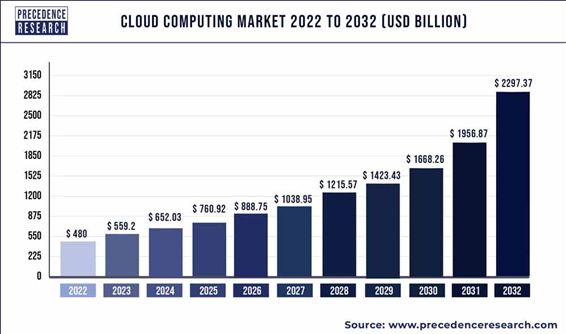
\includegraphics[width=\textwidth]{includes/images/precedence-research.png}
\captionvspace
\caption{Wykres przedstawiający prognozę wzrostu udziału rynkowego technologii chmurowej}
\label{fig:precedence-research}
\end{figure}

\section{Założenia i spodziewane wyniki}

Rezultatem niniejszej pracy dyplomowej jest rozebranie monolitycznego systemu na mikroserwisy z pojedynczą odpowiedzialnością logiczną. Zasada działa aplikacji nie ulega zmianie, dla użytkownika zewnętrznego wprowadzenie zmiany powinno odbyć się bez odczuwalnej różnicy. Samo rozczłonkowanie systemu odbywa jak najbardziej atomicznie się da przy rozsądnym nakłądzie pracy pozwalającym ukończyć tę pracę w terminie jej obrony. Autor zakłada, iż poprawie ulegnie bezpieczeństwo danych przechowywanych w bazie danych poprzez ukrycie bazy danych przed dostępem z zewnątrz przy wykorzystaniu wirtualnej sieci prywatnej, także większa granularność aplikacji poprawi bezpieczeństwo wdrożenia zmian poprzez ustystematyzowanie procesu jaki za tym stoi poprzez wykorzystanie technologii „Pipeline” (ciąg zautomatyzowanych procesów dostarczania nowego oprogramowania). Również autor odświeżył wersję zależności z jakich składa się projekt, tak by rozwiązać problemy luk bezpieczeństwa wynikających z użycia przestarzałych bibliotek. Dodatkowym poziomem ulepszenia zabezpieczeń aplikacji będzie przeszukanie kodu w pod kątem znalezienia luk logicznych lub twardo zakodowanych dostępów, takich jak hasła do bazy danych lub inne, z których aplikacja korzysta.

\chapter{Ewaluacja zastanej architektury aplikacji}

Zgodnie z stanem aplikacji z dnia 11.06.2022r. projekt “System do internetowego wspomagania pacjenta i lekarza” oparty jest o kilka składowych jakie należy wyróżnić, a są nimi:

\begin{itemize}
\item baza danych oprata o silnik MySQL,
\item trzon logiki biznesowej oparty o zestaw narzędzi Symfony w wersji 5.4,
\item warstwa widoku aplikacji oparta o silnik Twig oraz Vue.js,
\item silnik nginx jako narzędzie do przekazania zapytania klienckiego do logiki biznesowej.
\end{itemize}

Wyróżnione komponenty są ściśle ze sobą połączone. Logika biznesowa oraz baza danych są nierozerwalne, logika biznesowa posiada klasy encji, które bezpośrednio przekładają się na tabele w bazie danych. Logika biznesowa również decyduje o tym jaki widok jest obecnie wyświetlany, a warstwa widoku bazuje na tym, co dostarczył kontroler Symfony. Cały zestaw wykorzystuje narzędzie nginx do tego, by otrzymać zapytanie od klienta. W niniejszym rodziale zostaną przedstawione kolejno wyżej wymienione komponenty z szerszym opisem co do każdego z nich.

\section{Logika biznesowa i baza danych}

Symfony jako framework, który za zadanie ma ułatwić rozwój oprogramowania internetowego w projekcie z pracy inżynierskiej autora niniejszej pracy spełnił swoją rolę niejako przyczyniając się do skrócenia czasu potrzebnego na rzecz implementacji założeń diagramów użyć, odwzwierciedlenie domen każdego z aktorów systemu, a także diagramów przepływu danych. Narzędzia takie jak wbudowane kontrolery z dostępnym API do zapytań, czy formularze do walidacji danych wejściowych do systemu, router odpowiadający na zapytania, czy szablony wspierane przez silnik Twig to tylko niektóre z narzędzi jakie zostały wykorzystane przy okazji implementacji. Wyczerpujący schemat udogodnień oferowanych przez Symfony znajduje się na Rysunku~\ref{fig:symfony-metadata-scheme}.

\begin{figure}[ht]
\centering
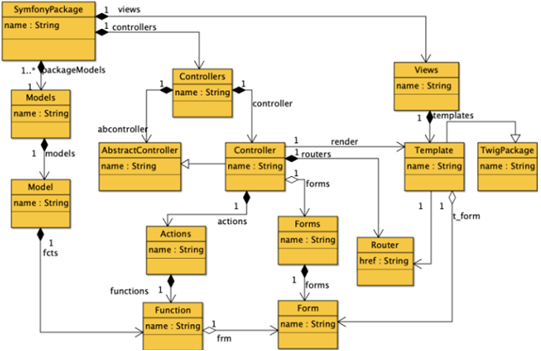
\includegraphics[width=\textwidth]{includes/images/symfony-metadata-scheme.png}
\captionvspace
\caption{Schemat metamodelu Symfony \cite{mod.driv.arch.symf}}
\label{fig:symfony-metadata-scheme}
\end{figure}

W celu odzwierciedlenia domen aktorów, w projekcie została wykorzystana biblioteka Doctrine, wspierana przez Symfony. Samo Doctrine to narzędzie do manipulacji bazą danych przy wykorzystaniu obiektów PHP \cite{symf.5}. By zainicjować dane w systemie bez konieczności manualnego wprowadzania ich autor wykorzystał dedykowaną ku temu bibliotekę wykorzystującą mechanizm fabryki danych testowych (ang. Fixtures Factory). Sam mechanizm fabryki danych testowych w procesie tworzenia oprogramowania umożliwia uruchomienie systemu z wypełnioną bazą danych, tak by móc przeprowadzać wymagane akcje i sprawdzić poprawność logiki biznesowej \cite{fixtures}.

\chapter{Planowanie architektury mikroserwisowej w chmurze AWS}
Niniejszy rozdział pokrywa zagadnienie planowania architektury mikroserwisowej oraz wykorzystanych usług potrzebnych do realizacji celu uruchomienia platformy. Nie istnieje mapa działań jakie należy wykonać by zgodnie z sztuką podzielić aplikację monolityczną na zbiór mikroserwisów. Istnieją natomiast wskazówki, którymi można się posługiwać by ułatwić doprowadzenie tego przedsięwzięcia do końca, a są nimi:

\begin{itemize}
\item identyfikacja mikroserwisów,
\item dbanie o szczególną troskę w procesie ekstrakcji modułów, które są kandydatami na mikroserwisy,
\item wprowadzenie modelu heksagonalnego aplikacji. \cite{java.ee.8.design.patterns}
\end{itemize}

\section{Wybór odpowiednich usług do utrzymania aplikacji}
W wyborze usług potrzebnych do użycia dla architektury mikroserwisowej, autor korzystał z własnych doświadczeń w pracy z platformą AWS. W związku z powyższym powody wyboru konkretnej usługi zostaną przedstawione w podrozdziale poświęconym na rzecz opisania motywacji doboru.

\subsection{Amazon VPC - Virtual Private Cloud (ang. prywatna, wirtualna chmura)}
Powody wyboru VPC dla celu realizacji architektury sieciowej:

\begin{itemize}
\item możliwość tworzenia wyizolowanych sieci w chmurze, co zapewnia wysoki standard bezpieczeństwa dla systemu, pozwala kontrolować ruch sieciowy przy pomocy reguł zapory sieciowej,
\item możliwość kontrolowania adresacji IP, podsieci, tabel routingu i bram internetowych, co pozwala na dostosowanie sieci do indywidualnych potrzeb budowanego przez autora systemu. \cite{aws.vpc}
\end{itemize}

\subsection{Amazon ECS - Elastic Container Service (ang. elastyczny serwis kontenerów)}
Wybór ECS jako usługi pozwalającej na uruchomienie mikroserwisów jest uargumentowany niniejszymi powodami:

\begin{itemize}
\item ułatwione zarządzanie kontenerami poprzez wbudowane narzędzia do orkiestracji nimi,
\item możliwość uruchomienia kontenerów bez konieczności zarządzania architekturą serwerową. \cite{aws.ecs}
\end{itemize}

\subsection{Amazon RDS - Relational Database Service (ang. zarządzany serwis relacyjnych baz danych)}
RDS jest idealnym wyborem do zarządzania bazami danych z następujących powodów:

\begin{itemize}
\item automatyzuje zadania typu tworzenie kopii zapasowych, aktualizacje oprogramowania oraz monitorowanie,
\item posiada rozwiązania gwarantujące wysoką dostępność,
\item oferuje szyfrowanie danych w spoczynku i w trakcie przesyłania oraz przy wykorzystaniu VPC do wyizolowania usługi zapewnia wysoki poziom bezpieczeństwa. \cite{aws.rds}
\end{itemize}

\subsection{Amazon MQ - Amazon Managed Message Broker Service  (ang. zarządzany broker komunikatów dostarczany przez Amazon)}
Z racji wykorzystania protokołu AMQP w projekcie migracji systemu, Amazon MQ jest odpowowiednim wyborem do zarządzania komunikacją między mikroserwisami z następujących powodów:

\begin{itemize}
\item umożliwia zautomatyzowanie konfiguracji, skalowania i zarządzania infrastrukturą brokerską,
\item obsługuje popularne protokoły wiadomości, takie jak: AMQP, MQTT oraz STOMP, najbardziej kluczowym dla aplikacji systemu do internetowego wspomagania pacjenta i lekarza jest AMQP,
\item posiada wbudowane mechanizmy redundancji i automatycznego przełączania awaryjnego,
\item oferuje szyfrowanie danych oraz izolację środowiska w VPC. \cite{aws.mq}
\end{itemize}

\subsection{Amazon IAM - Identity and Access Management (ang. zarządzanie tożsamością i dostępem)}
Najważniejszymi powodami do wyboru IAM jako usuługi zarządzającej dostępem są:

\begin{itemize}
\item precyzyjne zarządzanie dostępem do wszystkich zasobów AWS,
\item umożliwienie definiowania szczegółowych polityk uprawnień dla użytkowników, grup i ról,
\item zapewnia wysoki poziom bezpieczeństwa poprzez funkcje takie jak dwuskładnikowe uwierzytelnianie (MFA), tymczasowe poświadczenia oraz możliwość monitorowania działań użytkowników,
\item IAM udostępnia centralne zarządzanie tożsamościami i uprawnieniami, przez co upraszcza administrację i dodaje przejrzystości zarządzania dostępem. \cite{aws.iam}
\end{itemize}

\subsection{Amazon S3 - Simple Storage Service (ang. prosty magazyn danych)}
Przechowywanie danych aplikacji to kluczowe zadanie, jakie zostało postawione usłudze S3, a jej wybór został podyktowany następującymi powodami:

\begin{itemize}
\item usługa ta automatycznie skaluje się w górę lub dół, przez co umożliwia praktycznie nieograniczone ilościowo składowanie danych,
\item oferuje wysoką trwałość danych na poziomie bliskim 100\%, a także wysoką dostępność,
\item zapewnia szyfrowanie danych, zarządzanie dostępem na poziomie obiektu oraz integrację z AWS IAM,
\item umożliwia optymalizację kosztów na podstawie częstotliwości dostępu do danych i wymagań dotyczących trwałości. \cite{aws.s3}
\end{itemize}

\subsection{Amazon CloudWatch}
Usługa o nazwie CloudWatch, w szerokim spektrum usług jakie oferuje platforma AWS, dedykowana jest monitorowaniu i logowaniu akcji wykonanych w samych usługach, jak i w kodzie aplikacji. To są powody jakie zostały uwzględnione przy podjęciu decyzji o skorzystaniu z niej:

\begin{itemize}
\item umożliwia centralne zarządzanie i analizę danych,
\item oferuje zaawansowane możliwości monitorowania aplikacji i infrastruktury, a także konfigurację alarmów, które powiadamiają o problemach w czasie rzeczywistym,
\item na podstawie logów zbieranych przez CloudWatch, można zautomatyzować uruchamianie akcji skalowania zasobów, czy też funkcji Lambda. \cite{aws.cloud.watch}
\end{itemize}

\subsection{Amazon Route 53}
Jako, iż system modernizowany przez autora niniejszej pracy dyplomowej jest aplikacją internetową, to należy zapewnić mu dostęp do domeny, która będzie propagowoać jego usługi na cały świat. Usługą, w portfolio AWS, która zapewnia takie rozwiązania jest Amazon Route 53. Poniżej przedstawione są najważniejsze powody, które zostały uwzględnione przy dokonaniu wyboru:

\begin{itemize}
\item wysoka dostępność i niezawodność gwarantowane przez rozproszenie usługi DNS,
\item elastyczność i skalowalność,
\item zintegrowane funkcje geolokalizacji,
\item integracja z innymi, ważnymi z punktu widzenia systemu usługami, takimi jak: Elastic Load Balancing i CloudFront. \cite{aws.route53}
\end{itemize}

\subsection{Amazon Elastic Load Balancing}
Oferowana przez firmę Amazon usługa Elastic Load Balancing (ang. elastyczne balansowanie obciążeniem) jest kluczowym elementem każdej aplikacji z uwagi na rozproszenie obciążenia systemu. Niżej przedstawiono wszystkie powody wykorzystania omawianej usługi:

\begin{itemize}
\item automatycznie rozkładanie ruchu sieciowego między wieloma zasobami,
\item poprawa dostępności aplikacji poprzez monitorowanie stanu zasobów i automatyczne przekierowanie ruchu do zdrowych instancji,
\item zarządzanie ruchem na podstawie zawartości, geolokalizacji i opóźnienia między żądanym zasobem,
\item integracja z AWS Certificate Manager do zarządzania certyfikatami SSL/TLS, a także ochrona przez atakami DDoS i zarządzanie ruchem HTTP/2,
\item integracja z usługą Auto Scaling (ang. automatyczne skalowanie) oraz CloudWatch. \cite{aws.elb}
\end{itemize}

\subsection{ACM - AWS Certificate Manager (ang. menadżer certyfikatów AWS)}
Narzędzie ACM to natywne rozwiązanie chmury AWS oferujące szereg udogodnień istotnych z punktu widzenia cyberbezpieczeństwa, a są nimi:

\begin{itemize}
\item automatyzacja procesu tworzenia, wdrażania i odnawiania SSL/TLS,
\item integracja z Elastic Load Balancing (ELB), Amazon CloudFront i API Gateway (ang. bramka API),
\item bezpłatne utrzymanie certyfikatów SSL/TLS dla domen zarządzanych przez AWS,
\item łatwość użycia poprzez uproszczenie procesu zarządzania certyfikatami dzięki intuicyjnemu interfejsowi. \cite{aws.acm}
\end{itemize}

\subsection{Amazon API Gateway (ang. Bramka API Amazon)}
Usługa Amazon API Gateway została stworzona z myślą o maksymalnym uproszczeniu tworzenia struktury API i łączenia zasobów w jedną całość. Autor niniejszej pracy dyplomowej wykorzystał ją, po uprzednim zgłębieniu jej zalet, a są nimi:

\begin{itemize}
\item integracja z Amazon Elastic Load Balancing,
\item zarządzanie ruchem poprzez mechanizm Throttiling Rules (ang. zasady tłumienia),
\item łatwość tworzenia API i jego wdrożenia,
\item monitoring operacji wykonywanych wewnątrz API. \cite{aws.api.gateway}
\end{itemize}

\section{Opracowanie planu migracji}
Migracja działającego systemu monolitycznego na architekturę mikroserwisów jest wyzwaniem. Wiąże się tym duży koszt wstępny jaki musi ponieść przedsiębiorstwo, by uruchomić szereg koniecznych procesów pozwalających przeprowadzić odpowiednio migrację. Samą migrację należy przeprowadzić w pełnej świadomości i po przeprowadzeniu uprzednio audytu opłacalności tego zabiegu. Zabieg ten wprowadza znaczne skomplikowanie do projektu i wymaga wykwalifikowanej kadry inżynierów, którzy będą w stanie zapewnić ciągłość działania aplikacji w fazach przejściowych, a przy okazji rozwijając nową funkcjonalność.
W niniejszej pracy dyplomowej migracja zostanie przeprowadzona na systemie hobbystycznym, a co za tym idzie jego ewentualna przerwa w działaniu nie zadziała destrukcyjnie na ewentualne przedsiębiorstwo, które mogłoby ponieść koszta niedziałającej platformy. 

\subsection{Domain-Driven Design}
W skrócie DDD. Nazwa ta w języku polskim oznacza nacisk na prowadzenie rozwoju oprogramowania w kontekście jakiejś domeny. Jest to filozofia, która ma pomagać rozwiązywać problemy budowy oprogramowania dla skomplikowanych domen \cite{patterns.principles.and.practices.of.ddd}.
To podejście zakłada podział systemu na komponenty oraz ich zachowania, aby te wiernie odzwierciedlały rzeczywistość. Po wstępnej fazie planowania obszarów systemu następuje przejście do fazy implementacji.

Zadaniem autora w niniejszej pracy dyplomowej było wykorzystanie potencjału jaki został stworzony w jego pracy inżynierskiej. Mianowicie w omawianej pracy system został podzielony w naturalny sposób pośród czterech aktorów, jakimi są: pacjent, lekarz, pracownik recepcji oraz pracownik administracji. W tego podziału wyłania się domena podziału. Każdy aktor ma swój zestaw czynności jakie w swojej domenie może wykonywać. Tak na przykład każdy użytkownik ma prawa do edycji swojego konta, usunięcia go, oraz podglądu danych jakie się w nim znajdują. Przyglądając się funkcjonalności wizyt wyłania się osobna zależność, która jest możliwa do wydzielenia z całości systemu, a dostęp mają do niej aktorzy tacy jak: pacjent, lekarz i pracownik recepcji. Każdy z aktorów ma też swój indywidualny zestaw danych, który jest niezależny od innego z aktorów, co kwalifikuje ten fakt na uwzględnienie go jako podział na cztery dodatkowe domeny. Osobną zależnością jest również sama wysyłka maili, która z punktu widzenia systemu jest istotna, ale bardzo mała porównując zakres czynności jakie wykonuje.

Dalsze działania wynikające z planowania będą bazować bezpośrednio na wytyczonym powyżej podziale. Sam podział nie jest nowy w kontekście całego systemu. Autor zgodnie z sztuką zbudował projekt, tak by w przyszłości móc go rozwinąć właśnie poprzez modyfikację w kierunku mikroserwisów.

\subsection{Zakres migracji}
Według autora książki “Monolith to Microservices“ należy zrozumieć w jakim zakresie szczegółowa ma być domena, którą próbuje się dzielić na mniejsze części, tak by było to rozsądne \cite{monolith.to.microservices}. Patrz Rysunek~\ref{fig:ddd-sdiwpil}.

\begin{figure}[ht]
\centering
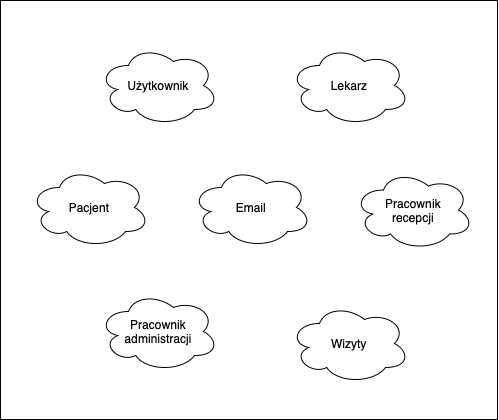
\includegraphics[width=\textwidth]{includes/images/ddd-sdiwpil.png}
\captionvspace
\caption{Zakres domenowy systemu do internetowego wspomagania pacjenta i lekarza}
\label{fig:ddd-sdiwpil}
\end{figure}

\subsection{Podejście Event Storming}
Podejście to polega na zgrupowaniu potencjalnych domen systemu za pośrednictwem akcji jakie wykonują. Tak na przykład w systemie do internetowego wspomagania pacjenta i lekarza da się pogrupować czynności wykonywane w systemie pod kątem wysyłki wiadomości e-mail. Na (Wstaw referencję obrazka) widoczny jest schemat pokazujący, że poszczególne domeny, takie jak: użytkownicy, wizyty są zgrupowane do akcji wysyłania wiadomości drogą mailową. Całość potencjału omawianego podejścia została przedstawiona na Rysunku~\ref{fig:event-storming-approach}.

\begin{figure}[ht]
\centering
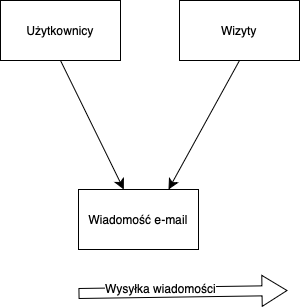
\includegraphics[width=\textwidth]{includes/images/event-storming-approach.png}
\captionvspace
\caption{Wysyłka wiadomości jest logicznie połączona dla tego modelu domeny, więc jej dalsza ekstrakcja może być trudna}
\label{fig:event-storming-approach}
\end{figure}

\chapter{Przebieg migracji}
W niniejszym rozdziale autor pracy dyplomowej przedstawił przebieg migracji, dzieląc go na osiem faz pośrednich. Przebieg ten jest odzwierciedleniem nakładu prac wykonanego przez autora na cel migracji systemu. Jest to połowa z potrzebnych działań praktycznych, ponieważ dalsza ich część to uruchomienie infrastruktury chmurowej w AWS.

\section{Faza pierwsza}
Po fazie planowania należy przejść do fazy, w której mając schemat podzielona zostanie całkowita migracja na fazy, tak by utrzymać ciągłość działania systemu. System uprzednio uruchomiony został w zwirtualizowanym środowisku Vagrant, gdzie miał zainstalowanie, które było proxy (ang. pośrednikiem) zapytań - nginx. W tym samym środowisku uruchomiony był również system do zarządzania relacyjną bazą danych - MySQL. Dodatkowo uruchomiona była tam również logika biznesowa przy pomocy gniazda PHP. Schematyczny obraz fazy pierwszej znajduje się na Rysunku~\ref{fig:migration-phase-1}.

\begin{figure}[ht]
\centering
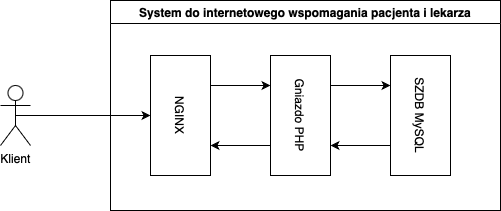
\includegraphics[width=\textwidth]{includes/images/migration-phase-1.png}
\captionvspace
\caption{Schemat architektury systemu do internetowego wspomagania pacjenta i lekarza w pierwszej fazie}
\label{fig:migration-phase-1}
\end{figure}

\section{Faza druga}
Wspieranym oprogramowaniem wirtualizującym na środowisku lokalnym i w samym AWS jest Docker. W drugiej fazie migracji wykonano opisanie bazy danych, pośrednika zapytań nginx i logiki biznesowej w osobnych, niezależnych kontenerach, skomunikowanych ze sobą wirtualną siecią. Omawiana zmiana widoczna na Rysunku~\ref{fig:migration-phase-2}.

\begin{figure}[ht]
\centering
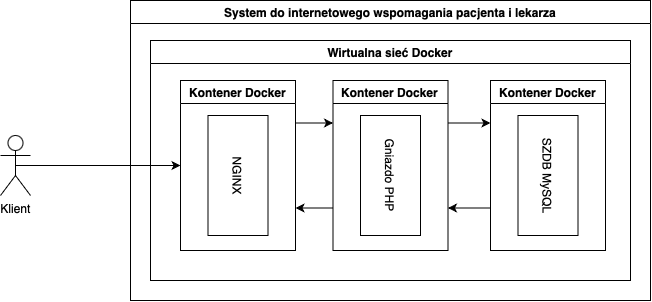
\includegraphics[width=\textwidth]{includes/images/migration-phase-2.png}
\captionvspace
\caption{Schemat architektury systemu do internetowego wspomagania pacjenta i lekarza w drugiej fazie}
\label{fig:migration-phase-2}
\end{figure}

\section{Faza trzecia}
W fazie trzeciej migracji systemu należy zacząć od domeny użytkownika i wydelegować ją do osobnego mikroserwisu od reszty monolitu, dodatkowo w samym monolicie należy poczynić zmiany, które uzależniają wszystkie czynności należące do zarządzania kontem użytkownika generycznego przetransferować by podlegały walidacji oraz wykonaniu przez mikroserwis. Na schemacie pojawia się zmiana nazewnictwa z “Gniazdo PHP” na “Monolit”, co od teraz symbolizować będzie całość logiki, ponieważ warstwa infrastruktury już nie jest istotna w tym momencie. Dodatkowo w oprogramowaniu pośredniczącym w zapytaniu między użytkownikiem a systemem - nginx należy poczynić zmianę konfiguracji, tak by ta przekazywała zapytania o użytkownika bezpośrednio do odpowiedniego kontenera z mikroserwisem w wirtualnej sieci Docker. W systemie do zarządzania relacyjną bazą danych należy utworzyć bazę danych odpowiadającą za tylko i wyłącznie dane wymagane do utrzymania w systemie przez mikroserwis użytkownika. Wyszczególniona powyżej zmiana została odzwierciedlona na Rysunku~\ref{fig:migration-phase-3}.

\begin{figure}[ht]
\centering
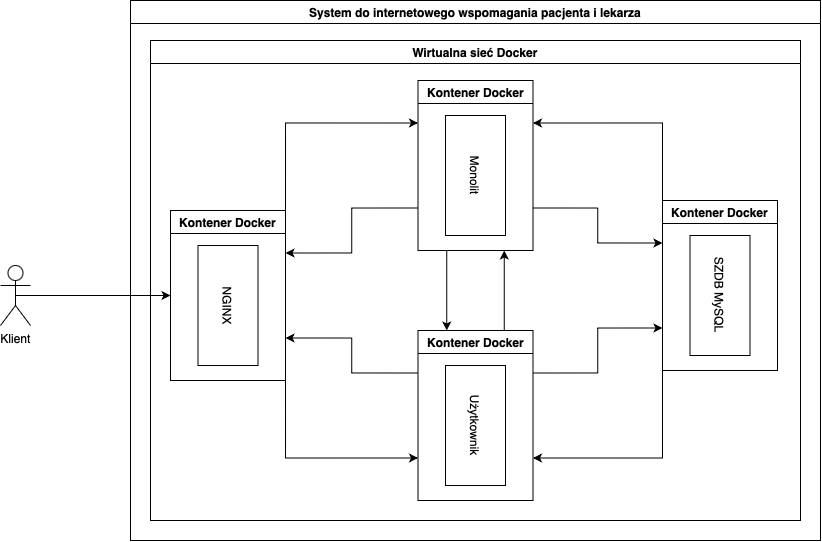
\includegraphics[width=\textwidth]{includes/images/migration-phase-3.png}
\captionvspace
\caption{Schemat architektury systemu do internetowego wspomagania pacjenta i lekarza w trzeciej fazie}
\label{fig:migration-phase-3}
\end{figure}

\section{Faza czwarta}
Faza czwarta migracji aplikacji zawiera w sobie dalszą modyfikację systemu. Początek zmian należy zawrzeć w konfiguracji oprogramowania nginx, gdzie należy przekierować cały ruch odpowiadający za obsługę użytkownika do mikroserwisu pacjenta. Dodatkowo utworzenie nowej bazy danych w systemie do zarządzania bazą danych MySQL. Niniejsza zmiana zwizualizowna została na Rysunku~\ref{fig:migration-phase-4}.

\begin{figure}[ht]
\centering
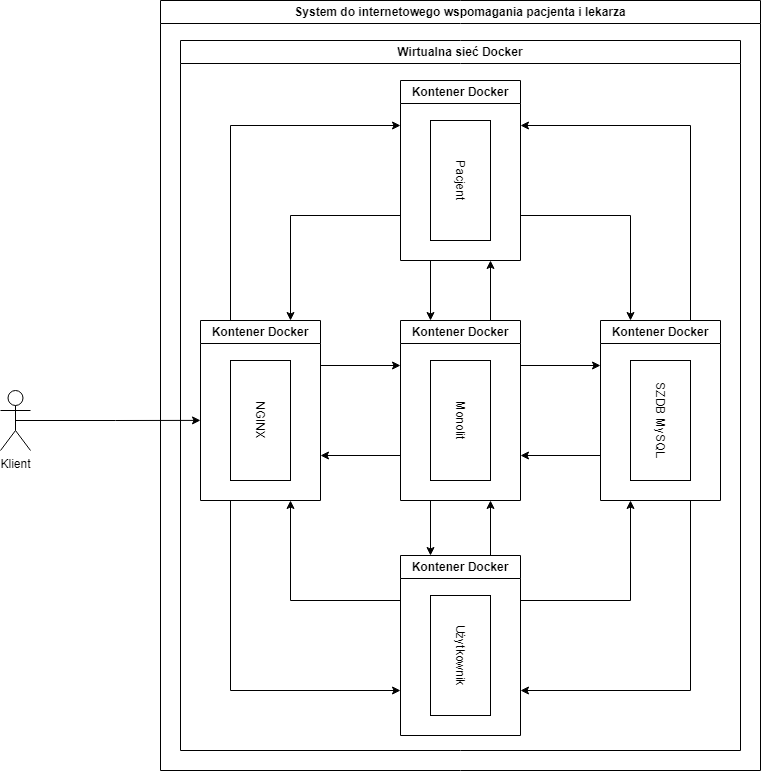
\includegraphics[width=\textwidth]{includes/images/migration-phase-4.png}
\captionvspace
\caption{Schemat architektury systemu do internetowego wspomagania pacjenta i lekarza w czwartej fazie}
\label{fig:migration-phase-4}
\end{figure}

\section{Faza piąta}
Kolejną fazą migracji jest część piąta, a ta będzie analogiczna do fazy czwartej. W jej skład będzie wchodzić utworzenie mikroserwisu dla pracownika recepcji oraz przekierowanie całego ruchu odpowiadającego za obsługę tej domeny do nowego mikroserwisu. Faza zostanie zakończona utworzeniem nowej bazy danych. Ta zmiana została przedstawiona na Rysunku~\ref{fig:migration-phase-5}.

\begin{figure}[ht]
\centering
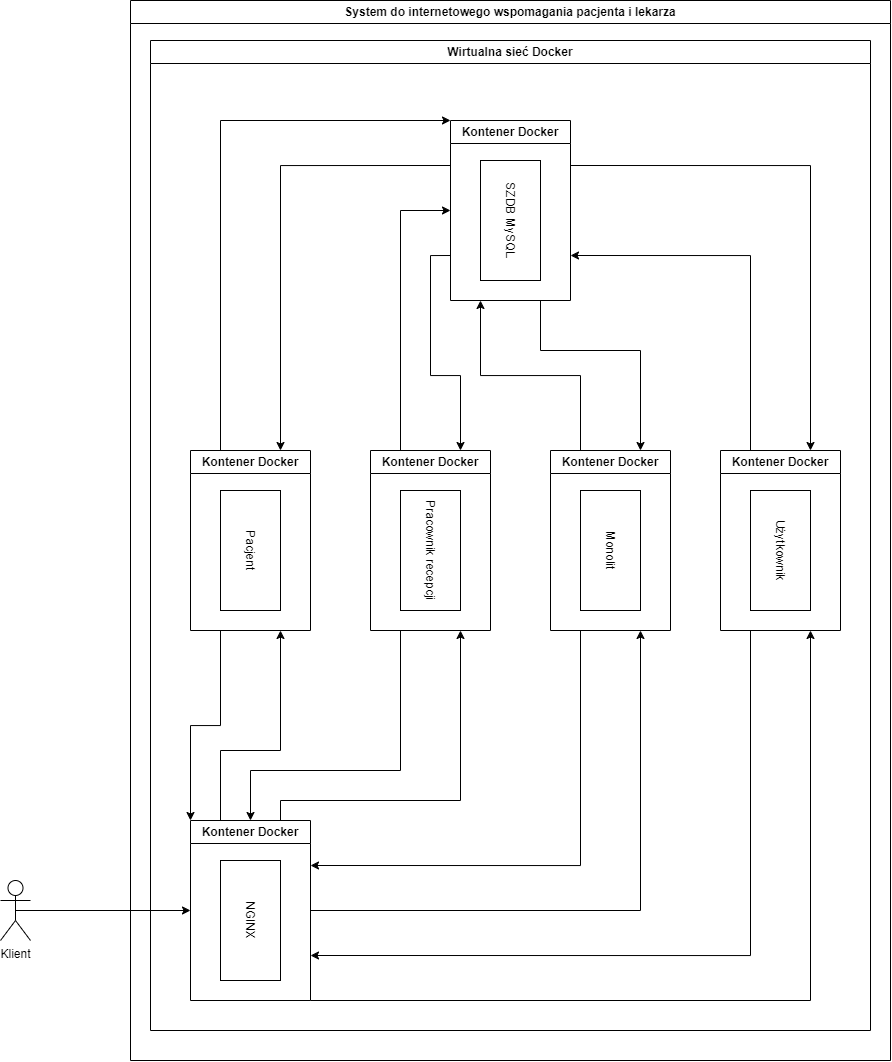
\includegraphics[width=\textwidth]{includes/images/migration-phase-5.png}
\captionvspace
\caption{Schemat architektury systemu do internetowego wspomagania pacjenta i lekarza w piątej fazie}
\label{fig:migration-phase-5}
\end{figure}

\section{Faza szósta}
W fazie szóstej dodano już ostatni mikroserwis odpowiadający za domeny związane z pracownikami lub użytkownikami. Utworzono zmiany w konfiguracji oprogramowania nginx oraz dodano bazę danych dla pracownika administracji. Zmiany zostały przedstawione na Rysunku~\ref{fig:migration-phase-6}.

\begin{figure}[ht]
\centering
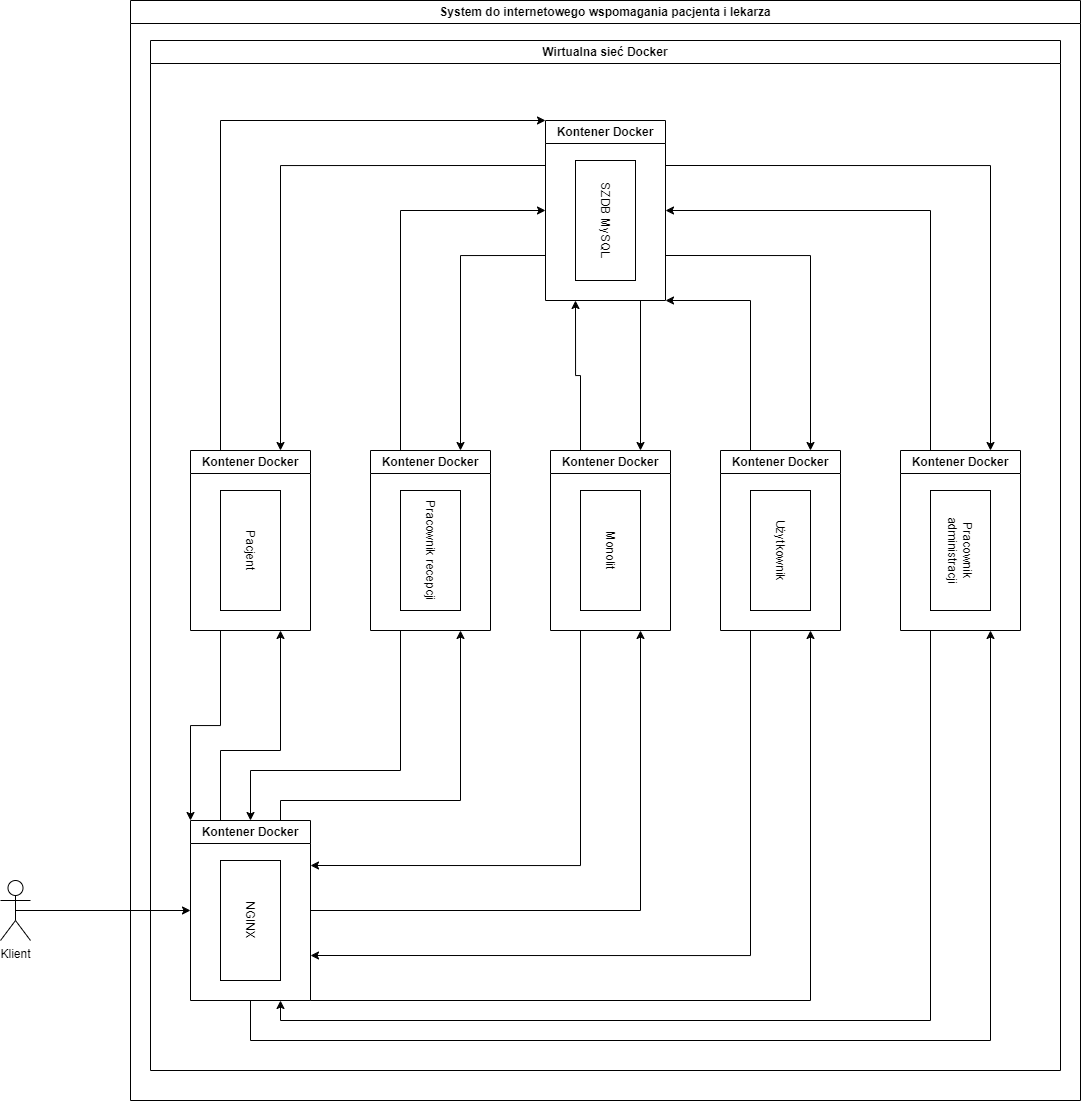
\includegraphics[width=\textwidth]{includes/images/migration-phase-6.png}
\captionvspace
\caption{Schemat architektury systemu do internetowego wspomagania pacjenta i lekarza w szóstej fazie}
\label{fig:migration-phase-6}
\end{figure}

\section{Faza siódma}
W fazie siódmej migracji dodano mikroserwis odpowiadający za obsługę wizyt. Proces technologiczny wygląda analogicznie do wcześniejszych faz. Wykonano zmianę konfiguracji oprogramowania nginx oraz utworzono nową bazę danych. Zmiany widoczne na Rysunku~\ref{fig:migration-phase-7}.

\begin{figure}[ht]
\centering
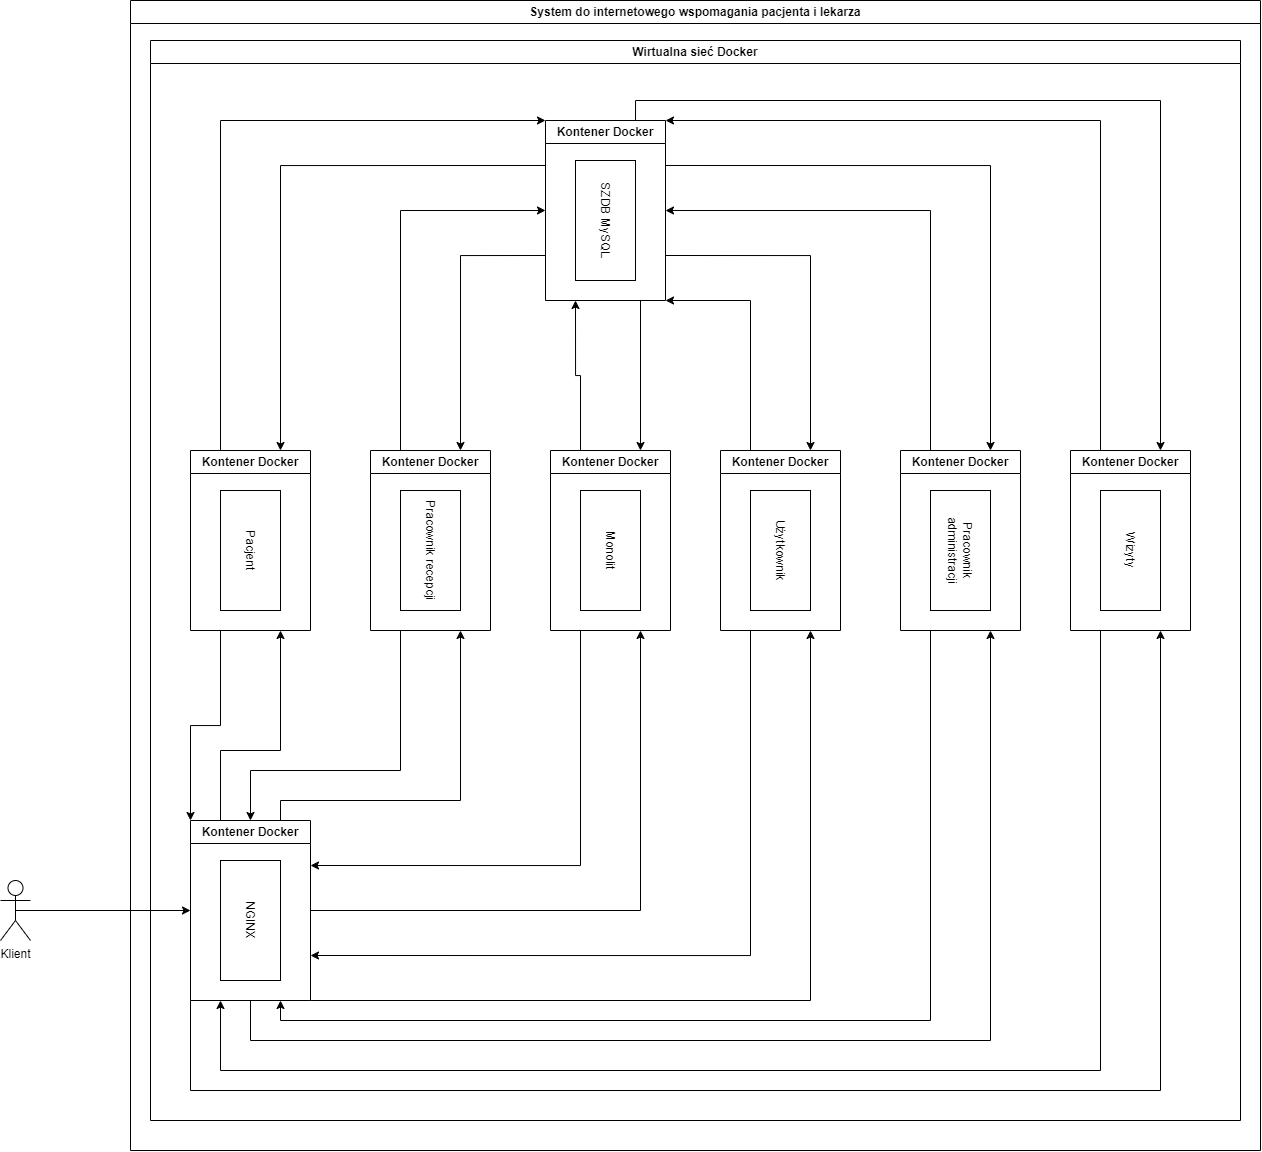
\includegraphics[width=\textwidth]{includes/images/migration-phase-7.png}
\captionvspace
\caption{Schemat architektury systemu do internetowego wspomagania pacjenta i lekarza w siódmej fazie}
\label{fig:migration-phase-7}
\end{figure}

\section{Faza ósma}
Ostatnia faza migracji to uruchomienie oprogramowania RabbitMQ, które będzie brokerem komunikatów portu AMQP. Dodatkowo uruchomiono serwis wysyłki maili. Na schemacie nastąpiło usunięcie części systemu określonej jako monolit, a to dlatego, że cały system w obecnym stanie jest już niezależny od jednej całości. Całość przedstawiona na Rysunku~\ref{fig:migration-phase-8}.

\begin{figure}[ht]
\centering
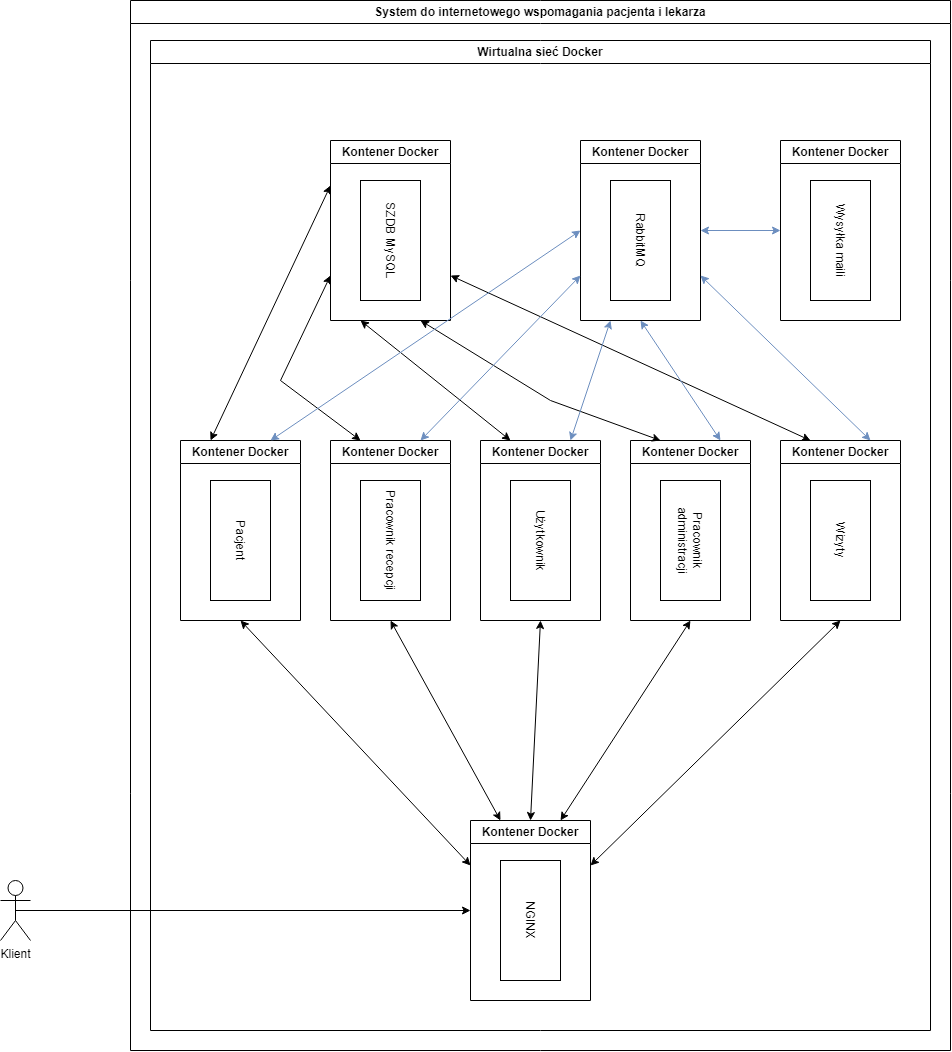
\includegraphics[width=\textwidth]{includes/images/migration-phase-8.png}
\captionvspace
\caption{Schemat architektury systemu do internetowego wspomagania pacjenta i lekarza w ósmej fazie}
\label{fig:migration-phase-8}
\end{figure}

\section{Podsumowanie przebiegu migracji}
Proces stopniowego ewoluowania projektu monolitycznego w projekt mikroserwisowowy dla systemu do internetowego wspomagania pacjenta i lekarza, jest procesem skomplikowanym. Czas poświęcony na dokonanie takiej migracji to w przybliżeniu 112h. Proces należał jednak do łatwiejszych przez wzgląd na niekomercyjne wykorzystanie systemu, a co za sobą wprowadza mniejsze ryzyko utraty danych lub poważnej awarii całej aplikacji.

\chapter{Bezpieczeństwo}

\section{Poziom zabezpieczeń przed migracją}
Niniejszy rozdział przedstawia stan poziomu zabezpieczeń przed migracją autora na system mikroserwisowy. Aspektem cechującym wszystkie systemy oparte o architekturę monolityczną jest fakt, że w przypadku awarii jednej usługi wewnątrz monolitu, niesie to ryzyko rozpropagowania awarii na cały system i zaburzenie jego działania. Ocena poziomu zabezpieczeń będzie krytyczna, ale złagodzona przez fakt, iż system nie działa w zakresie komercyjnym.

System do zarządzania bazą danych MySQL posiadał wyeksponowany na cały internet port, po którym potencjalny atakujący mógł przeprowadzić atak typu Brute Force w celu uzyskania dostępu do funkcji administracyjnych i potencjalnie pozyskanie danych przetrzymywanych w bazie danych. Atak typu Brute Force polega na próbie odgadnięcia hasła przez generowanie wszystkich możliwych kombinacji ciągu znaków. W teorii można złamać w ten sposób każde hasło \cite{brute.forcre}. Problem ten można rozwiązać na wiele sposobów, jednak autor tej pracy dyplomowej zastosuje ukrycie bazy danych w prywatnej sieci wewnętrznej, a dostęp do narzędzi administratorskich będzie się odbywać poprzez klucz SSH generowane przy pomocy algorytmów kryptograficznych takich jak RSA lub ECDSA.

Modernizowana aplikacja omawiana w tej pracy dyplomowej pierwotnie uruchomiona była na porcie HTTP 80, bez dodatkowych zabezpieczeń w postaci ważnego certyfikatu klucza publicznego. Certyfikat ten to informacja o kluczu publicznym podmiotu, która podpisana jest przez zaufaną stronę trzecią i jest niemożliwa do podrobienia \cite{pkn.ssl}. Wynikało to z faktu, iż dla celów akademickich nie istotnym było utworzenie owego certyfikatu i zadbanie o komunikację użytkownika poprzez szyfrowanych kanał na porcie HTTP 443. Kolejnym krokiem do przeprowadzenia odpowiedniej migracji mającej na celu uwzględnienie cyberbezpieczeństwo systemu jest dokonanie zmiany na komunikację szyfrowaną.

Ostateczne problemy wynikające z pomniejszego zaniedbania autora to fakt, iż system nie otrzymywał regularnych aktualizacji zabezpieczeń. W tym celu by zwiększyć poziom bezpieczeństwa należy uruchomić procedurę aktualizacji bibliotek zewnętrznych wykorzystywanych przez framework (ang. zestaw narzędzi) Symfony oraz także przeprowadzić aktualizację wersji interpretera języka programowania PHP. Ten sam fakt dotyczy również bibliotek, z których korzystała warstwa widoku pod postacią zestawu narzędzi Vue.js. 

\section{Bezpieczeństwo architektury chmurowej}
W dokumentacji narzędzia Amazon VPC podkreśla się, że dostarcza ono kluczowe rozwiązanie z punktu widzenia bezpieczeństwa każdego systemu opartego na obliczeniach chmurowych — izolację zasobów. Jest to możliwe dzięki logicznej izolacji wirtualnej sieci, którą definiuje użytkownik AWS. Narzędzie to oferuje również funkcje takie jak kreacja własnego zakresu adresów IP, tworzenie podsieci, konfiguracja tabel routingu oraz bramek internetowych, co pozwala na maksymalizację poziomu bezpieczeństwa i dostosowanie infrastruktury sieciowej do specyficznych potrzeb systemu.
Wyżej wymienione funkcje udostępnione przez Amazon w narzędziu VPC zostały częściowo wykorzystane przez autora niniejszej pracy dyplomowej. Obecne rozwiązania sieciowe są znacznie bardziej dostosowane do wymagań systemu do internetowego wspomagania pacjenta i lekarza w porównaniu z pierwotną konfiguracją.

Aspekt kontroli dostępu do zasobów w chmurze jest zarządzany za pomocą narzędzia Amazon IAM. Jest to podstawowy wybór w zakresie konfiguracji kontroli dostępu, od którego zależy określanie uprawnień. Na pierwszy rzut oka IAM może wydawać się skomplikowany, jednak po zapoznaniu się z jego dokumentacją i poradnikami, ukazuje swoją prostotę oraz przewagę, jaką zyskuje użytkownik konfigurujący zasoby swojego projektu z uwzględnieniem bezpieczeństwa. IAM oferuje bardzo szerokie spektrum konfiguracji — od ogólnych ustawień po najbardziej szczegółowe, co pozwala precyzyjnie określić uprawnienia osób, które potrzebują dokonać zmian.

Jedną z zalet tego rozwiązania jest możliwość tworzenia tymczasowych haseł dostępu, co umożliwia dynamiczne uruchamianie poszczególnych części infrastruktury lub automatyzowanie procesu wdrożenia, jeśli użytkownik konfigurujący dąży do utworzenia oprogramowania w podejściu IaaS (Infrastructure as a Service).

Dodatkowo narzędzie to posiada wbudowany program do analizy dostępu oraz walidacji skonfigurowanej polityki uprawnień. Program ten zamieszcza porady, jak efektywnie zmniejszyć uprawnienia, aby nie były one nadmierne, a jedynie pozwalały na wykonanie niezbędnych zadań \cite{aws.iam}.

\section{Bezpieczeństwo komunikacji}
Naturalnym aspektem wymiany danych pomiędzy poszczególnymi komponentami systemu modernizowanego przez autora pracy jest uwzględnienie szyfrowanej komunikacji. Efekt ten uzyskuje się poprzez wykorzystanie protokołów TLS/SSL, które zapewniają poufność i integralność przesyłanych danych. TLS wykorzystuje szyfrowanie asymetryczne.

Szyfrowanie asymetryczne to rodzaj kryptografii, w którym jeden z kluczy jest kluczem publicznym \cite{nature.tls.ssl}. Dowolny użytkownik może użyć tego klucza do zaszyfrowania wiadomości, jednak tylko posiadacz drugiego, prywatnego klucza może ją odszyfrować. W uproszczeniu, tak przebiega komunikacja z wykorzystaniem protokołu TLS/SSL.

Z perspektywy modelu OSI, będącego standardem komunikacji komputerowej zaproponowanym przez ISO, TLS odgrywa kluczową rolę w warstwie prezentacji, co pozytywnie wpływa na zabezpieczenie warstwy najwyższej — warstwy aplikacji. W przypadku systemu modernizowanego przez autora, jest to warstwa związana z protokołem HTTP.

W gamie usług AWS, narzędziem zarządzającym i dostarczającym darmowe certyfikaty do szyfrowanej komunikacji jest AWS Certificate Manager (menedżer certyfikatów AWS). Usługa ta ułatwia centralne zarządzanie certyfikatami, zarówno tymi wygenerowanymi przez Amazon, jak i dostarczonymi z zewnątrz. Dodatkowo AWS Certificate Manager bezpiecznie przechowuje certyfikaty, co zwalnia użytkownika korzystającego z usług AWS z odpowiedzialności za weryfikację potencjalnych luk w zabezpieczeniach \cite{aws.acm}.


\bibliographystyle{plain}
\bibliography{bibliography.bib}
\listoffigures
\end{document}
